\documentclass{article}
\usepackage[utf8]{inputenc}
\usepackage[T1]{fontenc}
\usepackage{lmodern}
\usepackage{graphicx}
\usepackage[frenchb]{babel}
\usepackage{hyperref}
\usepackage[table,xcdraw]{xcolor}
\usepackage{float}

\newcommand{\info}{\texttt}

\title{Objet et développement d'applications - Design Patterns\\
Projet libre : BloodBowl}
\author{Elbert Noel \bsc{NYUNTING} \and Corentin \bsc{CHÉDOTAL}}
\date{19 Novembre 2016}

\begin{document}

\maketitle

\centerline{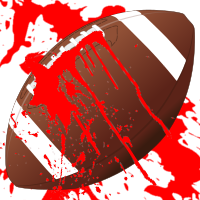
\includegraphics[scale=0.75]{img/logo.png}}

\begin{abstract}
    Dans le cadre de l'UE X5I0010 "Objet et développement d'applications" nous avons réalisé ce projet. Il comporte comme demandé plusieurs "designs patterns". Ont été utilisé les patterns [...]. Ce rapport expliquera leur implémentation, le but et fonctionnement du projet ainsi que les difficultés rencontrées dans la réalisation de celui-ci.
\end{abstract}

\tableofcontents

\section{Introduction}

\section{Le projet}

    \subsection{Description du projet et de son fonctionnement}
    %INSERER DIAGRAMME COMPLET

    \subsection{Principales classes}

        \subsubsection{Classe Poney}

    \subsection{Design patterns employés}

        \subsubsection{Design Strategy}
        %INSERER DIAGRAMME
        
\section{Commentaires sur le projet}

    \subsection{Difficultés recontrées}
    
    \subsection{Autres}

\end{document}

